% !TEX root = ../main.tex
% chktex-file 21
% chktex-file 46
\section{Effects of Coarsening}%
\label{sec:cons}

We have just seen how to compute a coarsened graph $G_c$ via the REC algorithm.
What remains to be answered now is how coarsening affects the performance of graph algorithms when $G_c$ is used as a proxy for the original graph $G$.
In the first step we will introduce a graph similarity measure.
Using this measure we will then put bounds on the dissimilarity of $G$ and $G_c$.
Finally we will use those bounds to analyze the influence of coarsening on the performance of the \textit{spectral clustering algorithm}.

\subsection{Restricted Spectral Similarity}%
\label{sec:cons:rss}

To compare a graph $G$ with its coarsened version $G_c$ we will use the notion of \textit{spectral similarity}.
As we have seen before, $G$ can be viewed as an operator that transforms an input signal $x \in \mathbb{R}^N$.
We described this transform in terms of the graph's Laplacian $L$,
more specifically in terms of the Laplacian's eigenbasis ${\{ u_k \}}_{1 \leq k \leq N}$ and spectrum ${\{ \lambda_k \}}_{1 \leq k \leq N}$.
Similarly the coarsened graph $G_c$ can be described in terms of its Laplacian $L_c$.
Since $L \in \mathbb{R}^{N \times N}$ and $L_c \in \mathbb{R}^{n \times n}$ act on signal spaces of different dimensionality, they cannot be compared directly however.
Instead we compare $L$ with $\widetilde{L} = C^{\top} L_c C$, the upsampled version of $L_c$.
We say $\widetilde{L}$ is an \textit{$\varepsilon$-approximation} of $L$ iff.\  $\widetilde{L}$ scales the eigenvectors $u_k$ of $L$ by a factor of roughly $\lambda_k$ in the direction of $u_k$:
\begin{wrapfigure}{r}{0.25\textwidth}
	\centering
	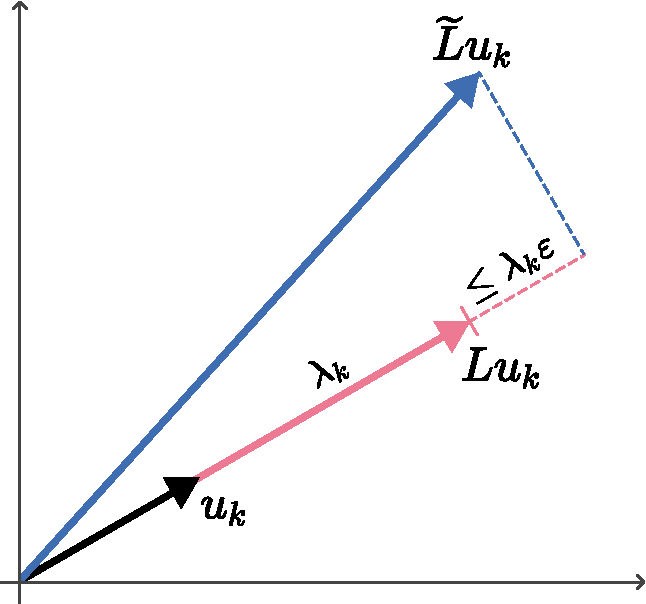
\includegraphics[width=\linewidth]{gfx/cons/rss.pdf}
	\caption{See \cref{eq:cons:rss}.}\label{fig:cons:rss}
\end{wrapfigure}
\begin{align}
	\forall k \leq K:\ (1 - \varepsilon) \underbrace{u_k^{\top} L u_k}_{\lambda_k} \leq u_k^{\top} \widetilde{L} u_k \leq (1 + \varepsilon) \underbrace{u_k^{\top} L u_k}_{\lambda_k} \text{ with } \varepsilon \geq 0\label{eq:cons:rss}
\end{align}
The reason we require \cref{eq:cons:rss} to hold only for the first $K$ eigenvectors of $L$ is, that $\text{rank}(L) = N - c$, whereas $\text{rank}(\widetilde{L}) = n - c$;
i.e.\ $\widetilde{L}$ has a higher dimensional null space\footnote{%
	Here $c$ denotes the number of connected components of $G$.
	They reduce the rank since $\lambda_1 = \cdots = \lambda_c = 0$.
}.
Thus \cref{eq:cons:rss} cannot hold for a signal $x$ that is in the null space of $\widetilde{L}$ but not in that of $L$.
Therefore the similarity condition is restricted to the first $K$ eigenvectors, as they represent the most important ``low-frequency'' components of $G$.
This restricted condition is called \textit{restricted spectral similarity} (RSS).

The choice of $K$ in RSS depends on the level of detail that should be considered when comparing $L$ and $\widetilde{L}$.
If $G$ has $c'$ clusters, i.e.\ connected subgraphs with relatively few edges going out of it, a choice of $K = c'$ is reasonable.
That way RSS checks whether the clusters of $G$ are preserved in the coarsened graph $G_c$ and how much the connectedness between the clusters changes.
Details like the connections within clusters on the other hand do not have a strong influence on the RSS similarity if $K = c'$, since they are described by the ``high-frequency'' eigenvectors $u_\ell$ of $L$ where $\ell > K$.

\subsection{Bounding REC via RSS}%
\label{sec:cons:bound}

Now we will use RSS to bound the eigenvalue error caused by REC coarsening.
It can be shown that the probability of satisfying the RSS condition for a single eigenvector $u_k$ with a sufficiently small eigenvalue $\lambda_k$ is lower-bounded by
\begin{align}
	P\mkern-2mu\left((1 - \varepsilon) \lambda_k \leq u_k^{\top} \widetilde{L} u_k \leq (1 + \varepsilon) \lambda_k\right)
	\geq 1 - \frac{r \nu_{\text{max}}}{2 \varepsilon d_{\text{avg}}} \left(1 + \frac{3 - 4 \lambda_k}{\nu_{\text{min}}}\right)\label{eq:cons:bound}
\end{align}
where $r = \mathbb{E}\mkern-2mu\left[\frac{N - n}{N}\right]$ is the expected graph reduction ratio, $d_{\text{avg}} = \frac{1}{N} \sum_{v_i \in \mathcal{V}} d_i$ is the average vertex degree and $\nu_{\text{min}}$/$\nu_{\text{max}}$ are the minimum and maximum of the neighborhood weights ${\{ d_i + d_j - w_{i j}  \}}_{e_{i j} \in \mathcal{E}}$.
For a formal proof of this bound we refer to \citet[Suppl.~2]{Loukas2018}.
Here we will instead focus on giving an intuition for its key implications:
\begin{enumerate}[label=\textbf{\arabic*.}]
	\item \textbf{The $\varepsilon$-term:}
		Unsurprisingly the RSS bound is inversely proportional to $\varepsilon$; relaxing the approximation bound makes it is more likely to be satisfied.
	\item \textbf{The $r$-term:}
		The RSS bound is linearly dependent on the reduction ratio $r$.
		The more the graph size is reduced, the smaller the probability of satisfying the bound.
	\item \textbf{The $\lambda_k$-term:}
		There is also a linear dependence on $\lambda_k$;
		for large eigenvalues the probability of satisfying the bound goes \textit{down}.
		This happens despite the fact that the associated eigenvectors $u_k$ represent ``high-frequency'' components of $G$ that are more easily disturbed than the smooth ``low-frequency'' eigenvectors.
	\item \textbf{$\nu_{\text{min}}$, $\nu_{\text{max}}$ and $d_{\text{avg}}$:}
\end{enumerate}
\begin{figure}[ht]
	\centering
	\begin{subfigure}{0.33\textwidth}
		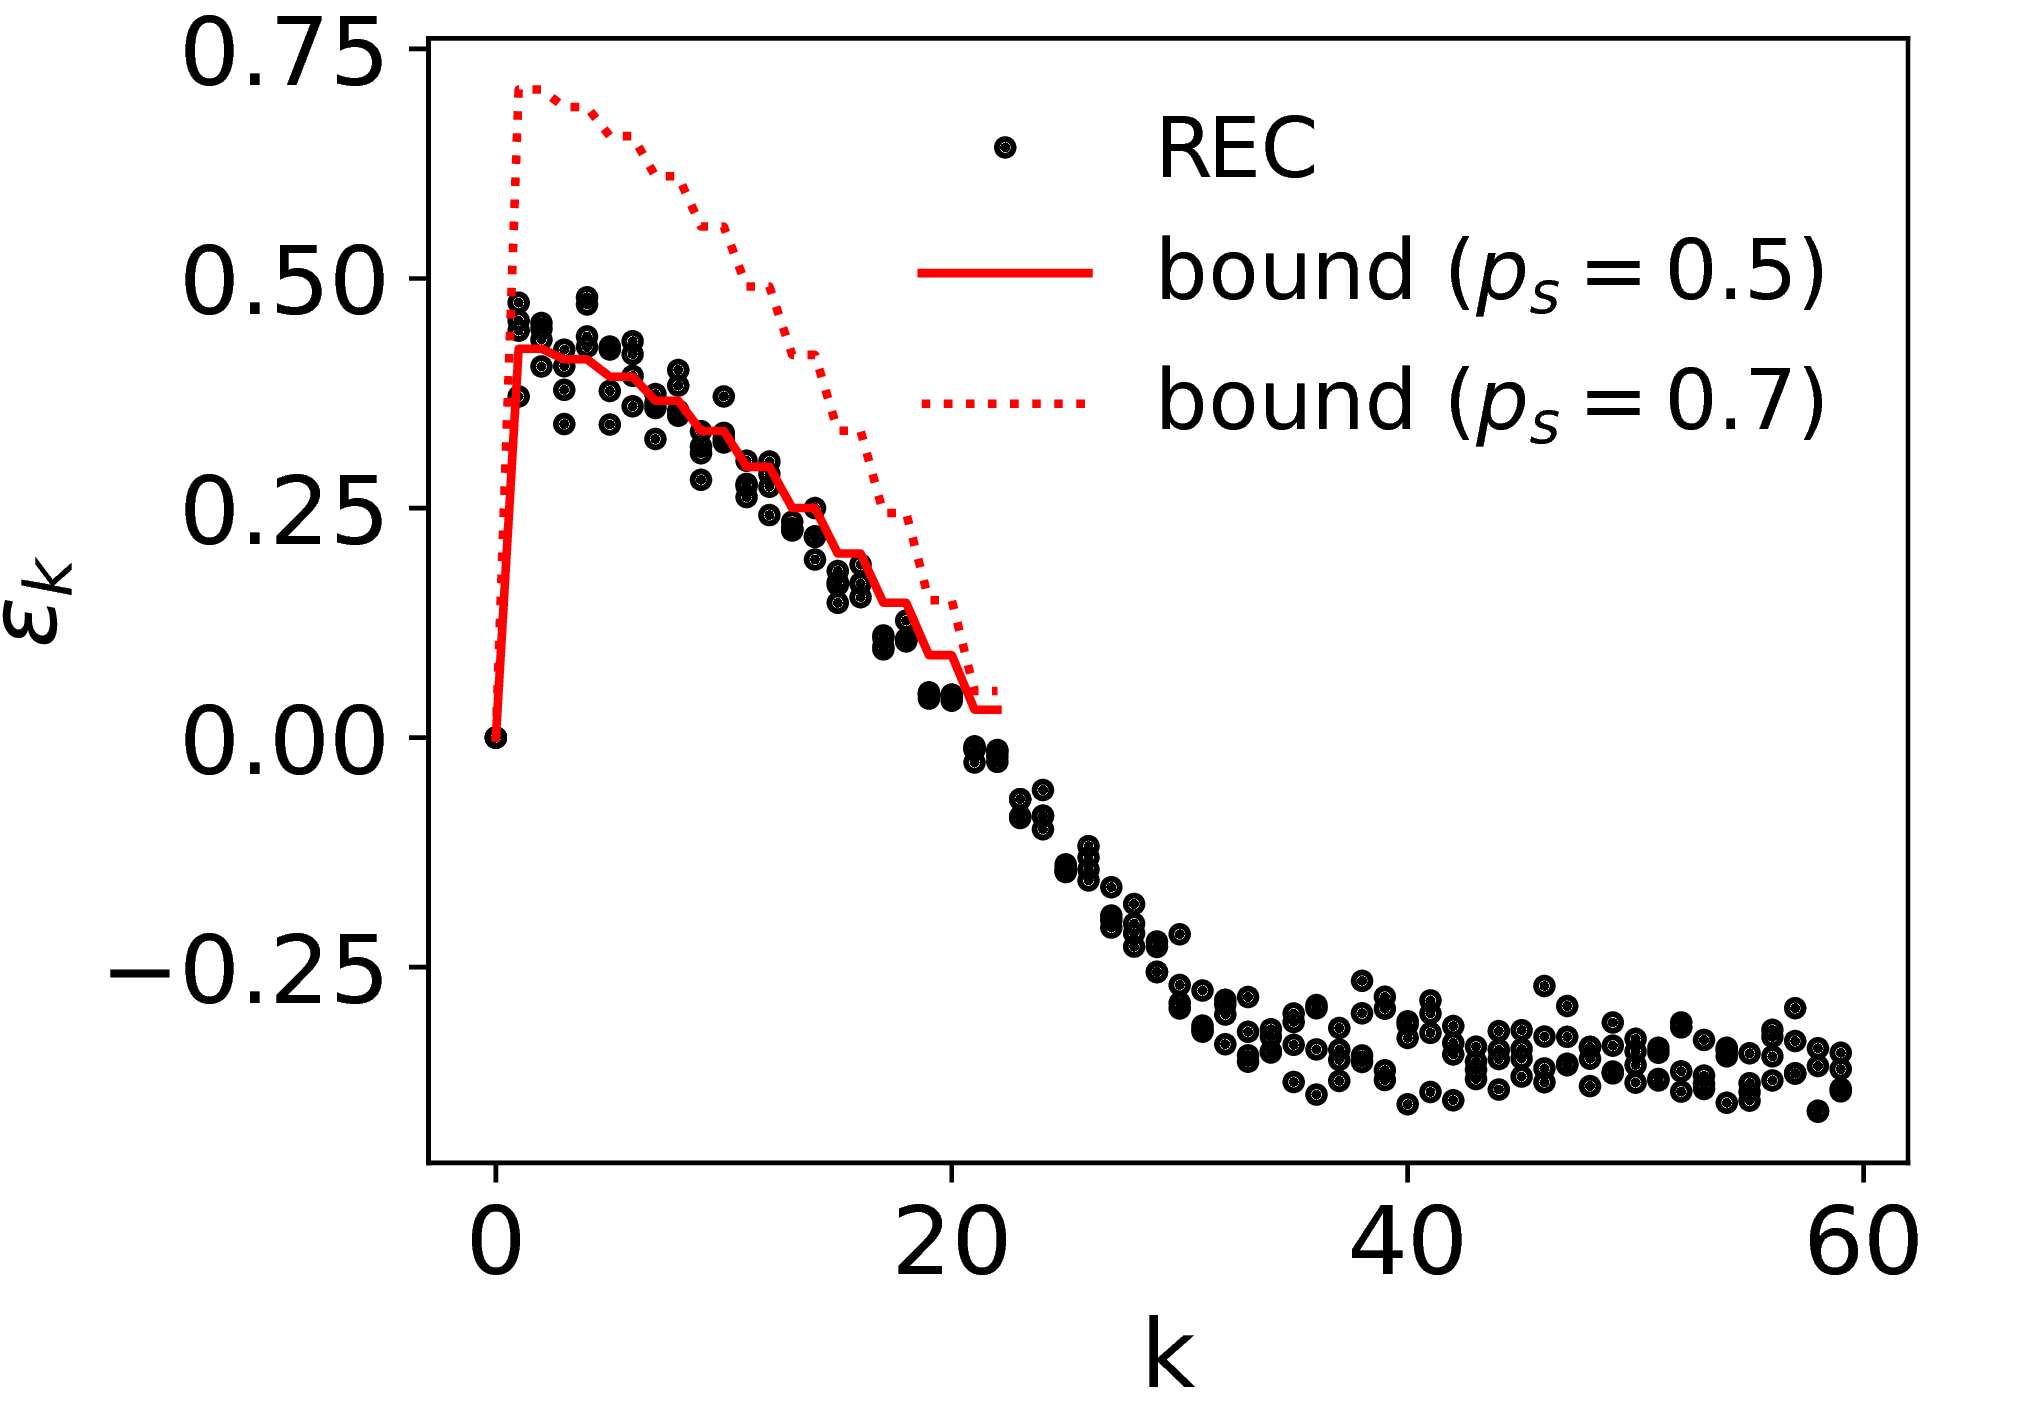
\includegraphics[width=\linewidth]{gfx/cons/example/regular.png}
		\caption{Regular graph ($d = 20$)}\label{fig:cons:example:regular}
	\end{subfigure}%
	\begin{subfigure}{0.33\textwidth}
		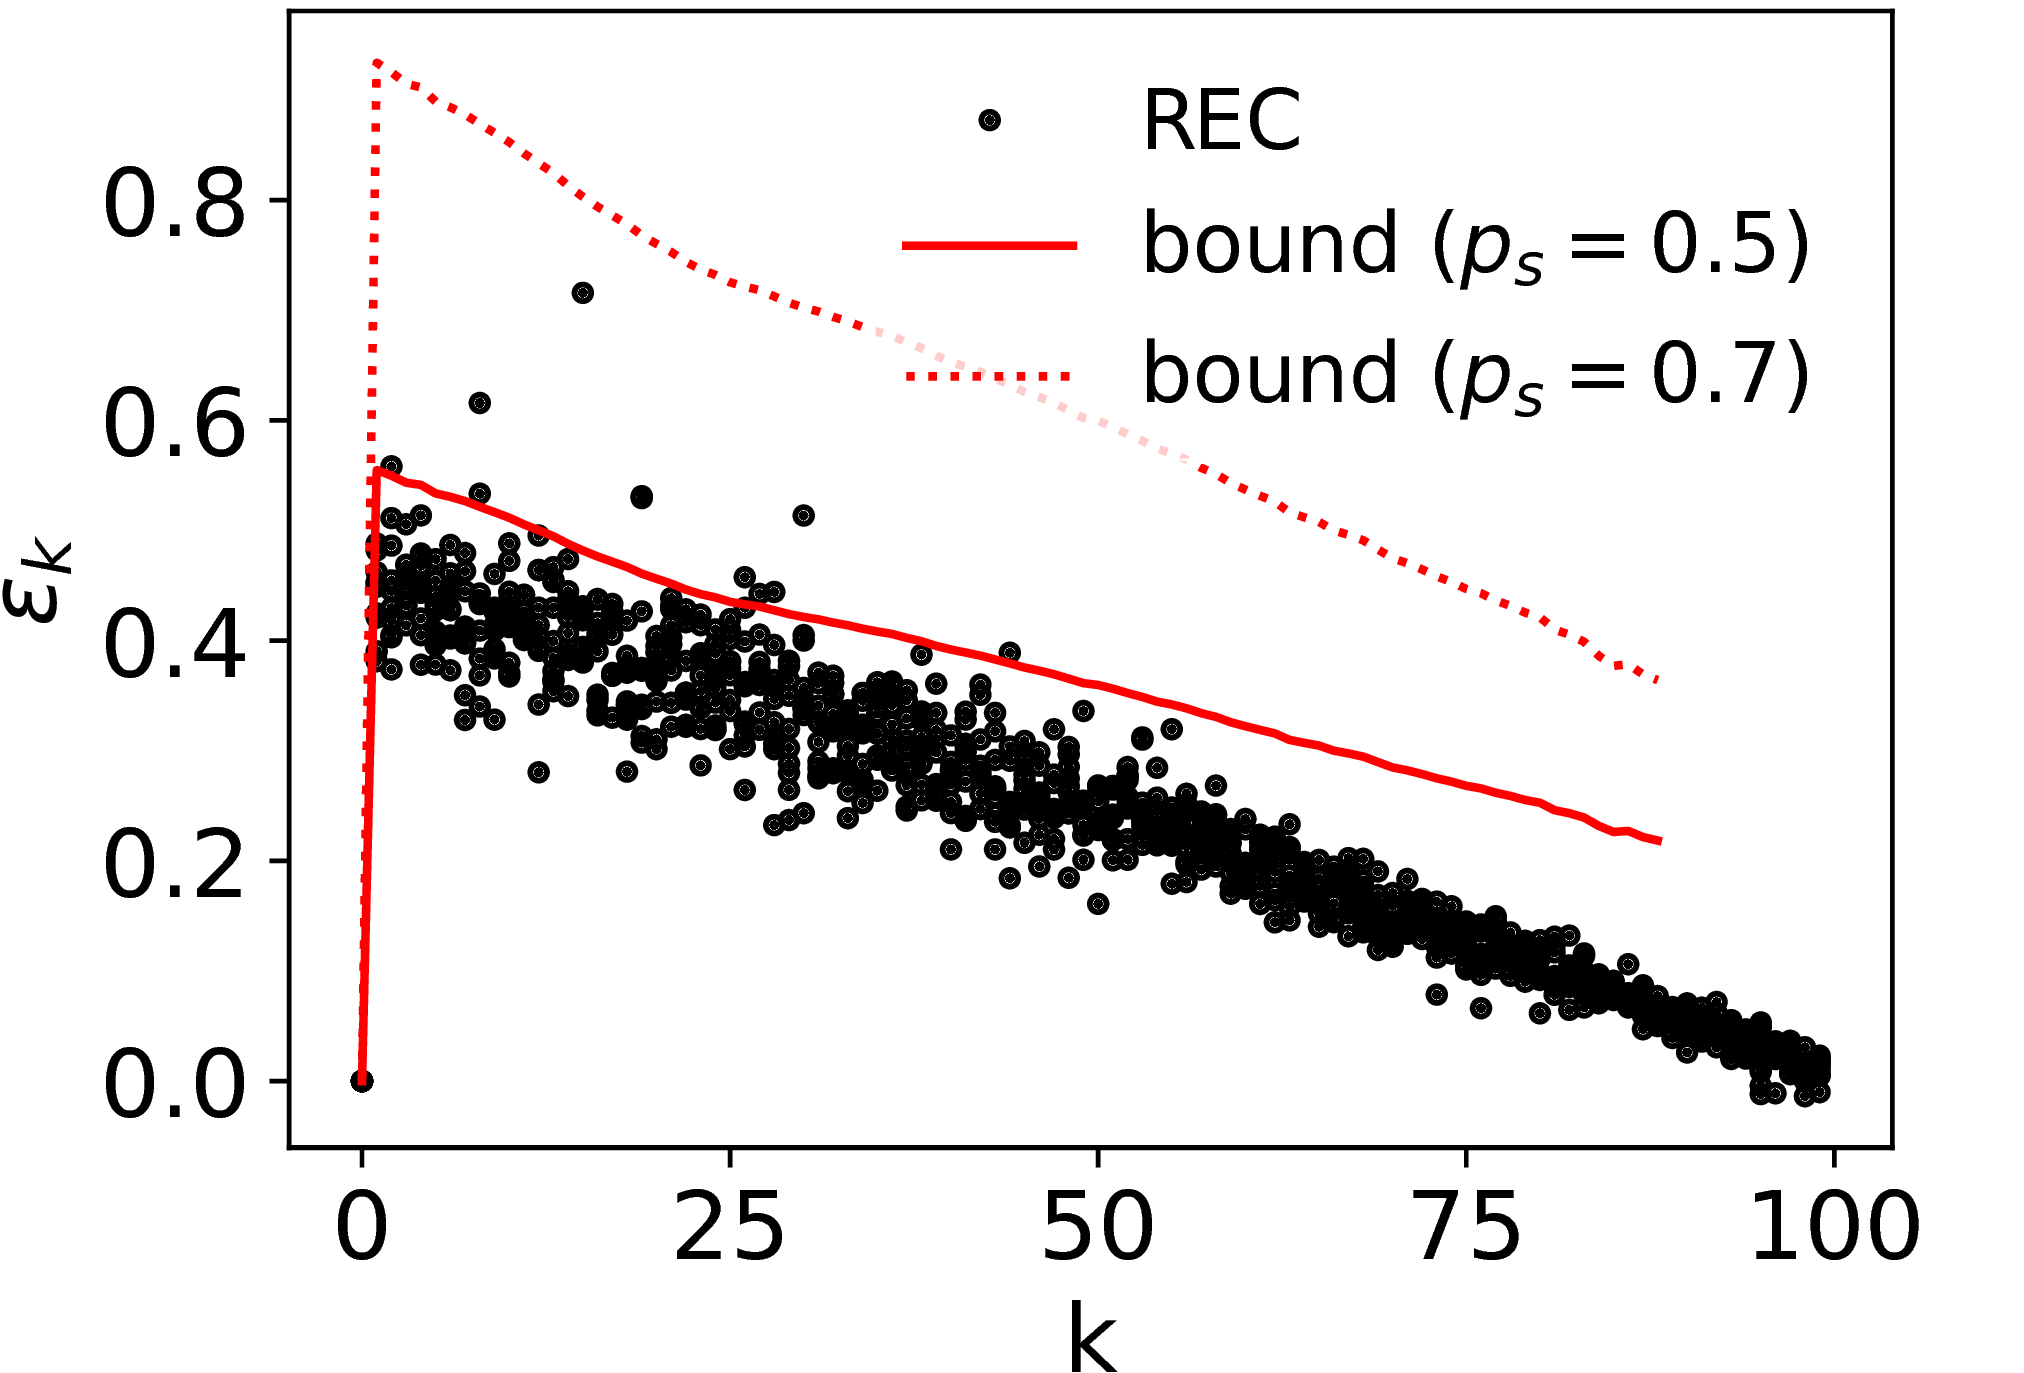
\includegraphics[width=\linewidth]{gfx/cons/example/yeast.png}
		\caption{Yeast (protein network)}\label{fig:cons:example:yeast}
	\end{subfigure}%
	\begin{subfigure}{0.33\textwidth}
		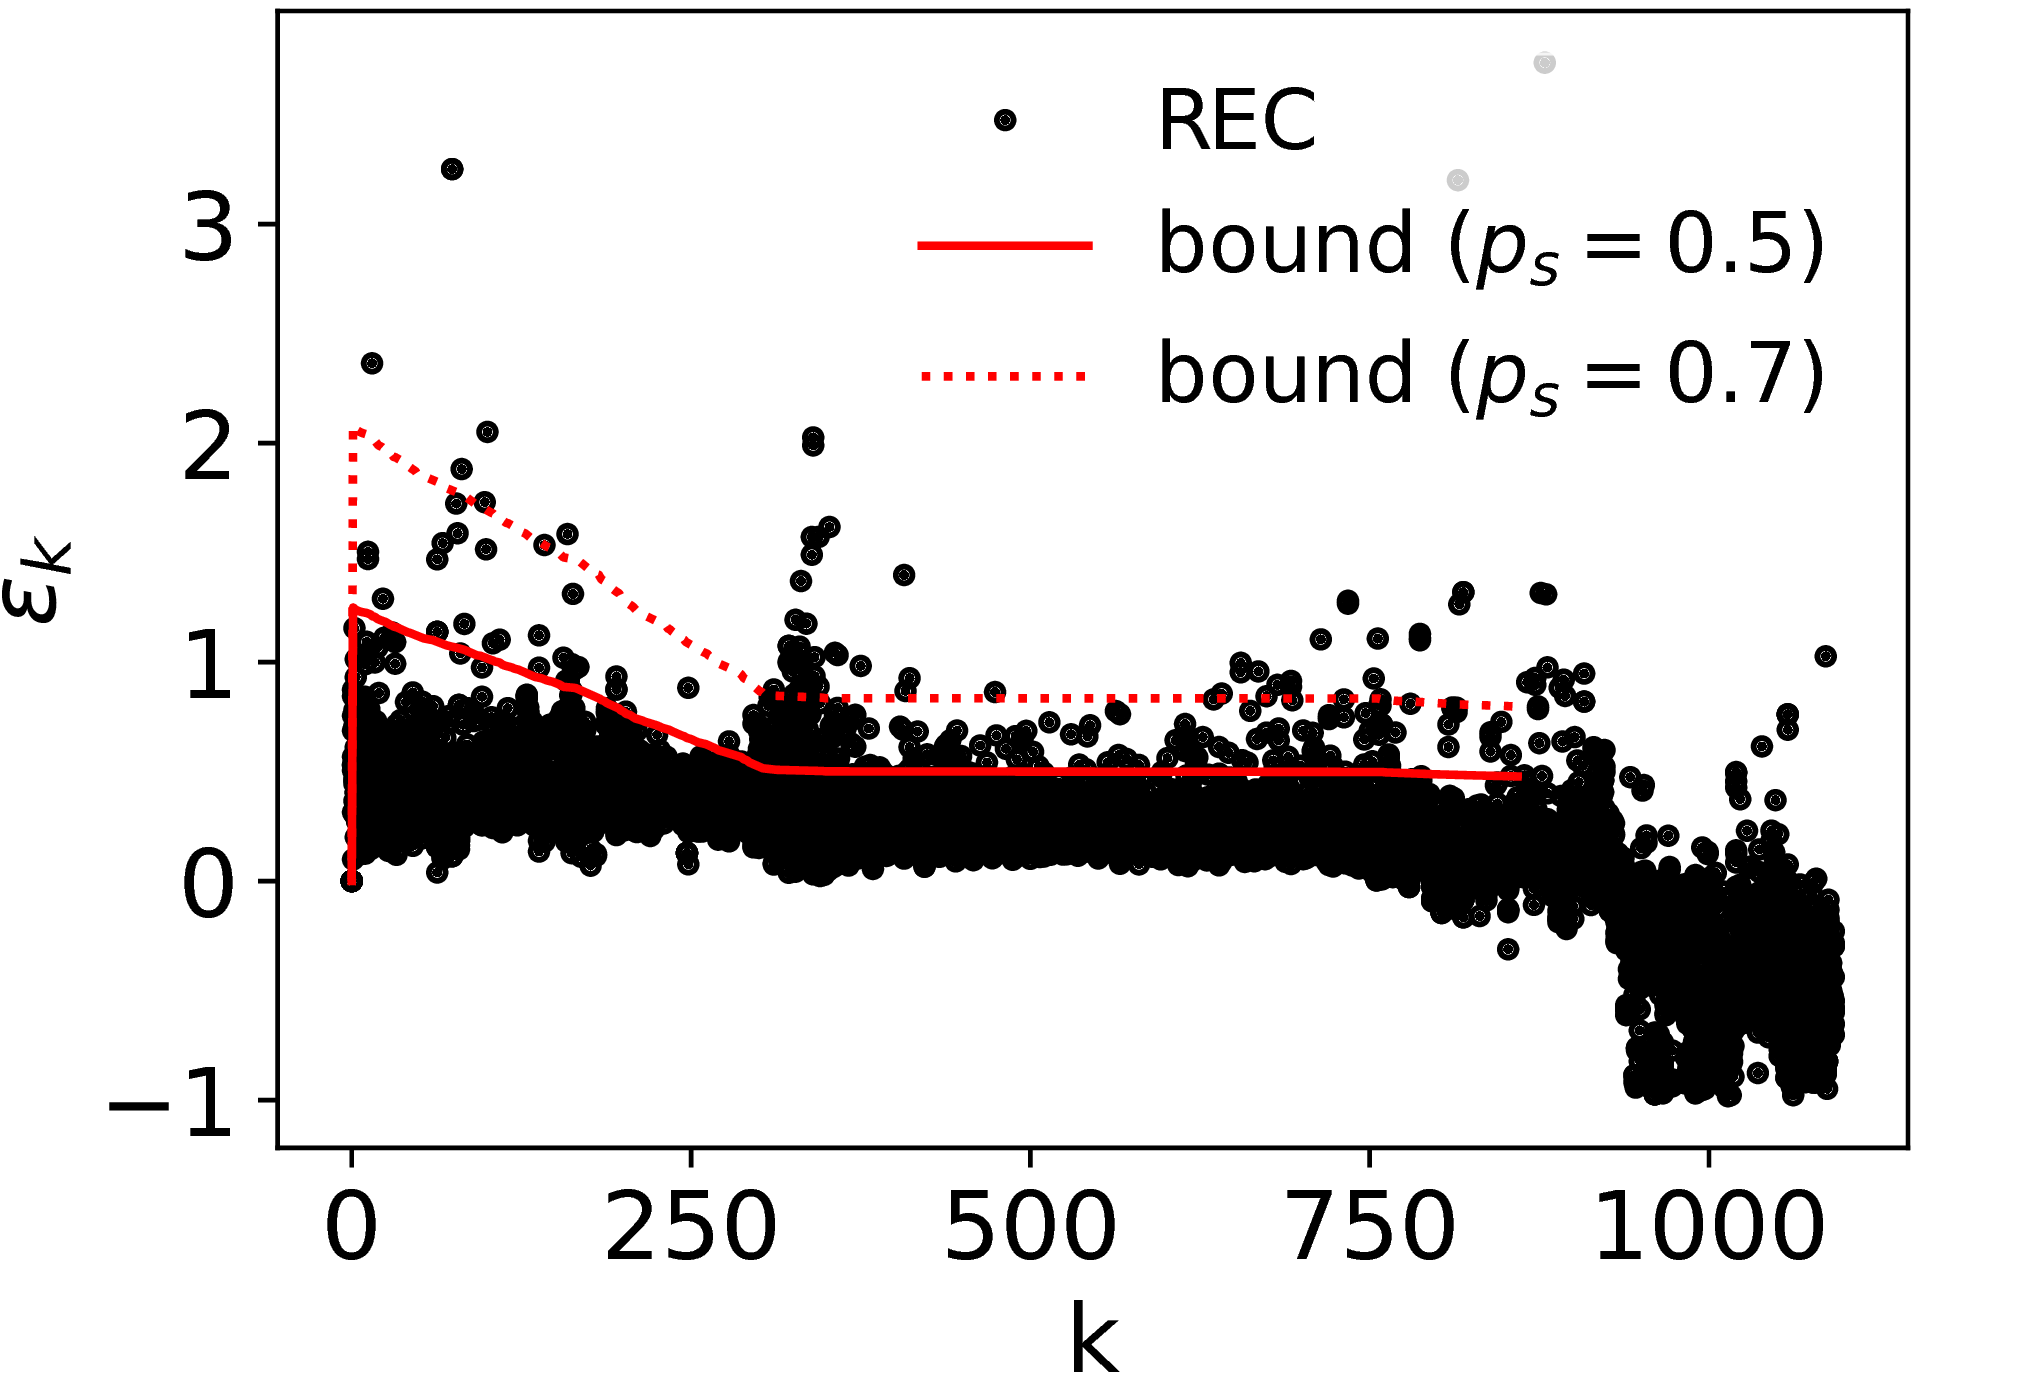
\includegraphics[width=\linewidth]{gfx/cons/example/roll.png}
		\caption{Swiss roll (manifold)}\label{fig:cons:example:roll}
	\end{subfigure}
	\caption{%
		Comparison of the RSS-bound and the actual error constants $\varepsilon$ for the eigenvectors of multiple coarsened graphs ($r = 0.4$).
		Confidence bounds for $p_s \in \{0.5, 0.7\}$ are shown.
	}\label{fig:cons:example}
\end{figure}

\subsection{Implications for Spectral Clustering}%
\label{sec:cons:sc}
